% Provenance (never printed): see sources/outline_sources.md (Year 1: gravity and its
% measurement, normal gravity; isostasy, Airy and Pratt; free-air and Bouguer anomalies;
% the geoid). Curves from figdata/bachelor-1/hypsometry.py and gravity_profiles.py;
% exercise and problem values in the Book 3 scratch calculator calc/ch11.py.
\chapter{समस्थिति और गुरुत्व विसंगतियाँ}\label{ch:b1:isostasy-gravity}

1840 के दशक में उत्तरी भारत में एक मध्याह्न-चाप मापते सर्वेक्षकों को एक ऐसा अंतर मिला जिसका दोष वे अपने उपकरणों पर नहीं डाल सकते थे। लगभग 370 मील दूर दो स्टेशनों, हिमालय की तलहटी के निकट कालियाना और दक्षिण में दूर कालियानपुर, के बीच त्रिकोणमिति से मिला अक्षांश-अंतर, तारों से मिले अंतर से 5.236 चाप-सेकंड अधिक था। स्पष्ट अपराधी पर्वत थे: उनका आकर्षण ओलंब-रेखा को उत्तर की ओर खींचता है, और खगोलविद अपने उपकरण ओलंब-रेखा से साधते थे। 1855 में जॉन हेनरी प्रैट ने हिमालय और उसके परे के पठारों के आकर्षण की गणना की और पाया कि इससे अंतर 15.885 सेकंड होना चाहिए था, जो प्रेक्षित से तीन गुने से भी अधिक है। पर्वत अपने दृश्य द्रव्यमान की अपेक्षा कहीं कम खींचते थे। उसी वर्ष जॉर्ज एयरी ने उत्तर दिया कि \omterm{def:b1:layered-earth:layers}{भूपर्पटी} एक सघनतर परत पर पानी में लकड़ियों के बेड़े की तरह तैरती है, इसलिए ऊँची भूमि की गहरी जड़ होती है जो हल्की चट्टान की होती है; प्रैट ने बाद में एक और उत्तर सुझाया, पर्वतों के नीचे विस्तार से हल्की हुई चट्टान। दोनों अब भी पढ़ाए जाते हैं: पर्वतों के नीचे हल्की चट्टान है जो उनके द्रव्यमान की भरपाई करती है। यह अध्याय उस विचार को संख्याओं में बदलता है, और दिखाता है कि गुरुत्व, जो अपने मान के एक दस-लाखवें भाग तक मापा जाता है, उच्चावच के नीचे छिपे द्रव्यमानों को कैसे प्रकट करता है।
% ledger: pratt:himalaya, airy:1855, pratt:1871

\begin{recall}
न्यूटन का गुरुत्वाकर्षण नियम $g = GM/r^2$ देता है, जो गोलीय द्रव्यमान $M$ के बाहर का क्षेत्र है; यह क्षेत्र एक गुरुत्वीय विभव से निकलता है, और एक समविभव पृष्ठ हर जगह क्षेत्र के लंबवत होता है (भौतिकी)। स्थिर द्रव में दाब $\mathrm dp/\mathrm dz = \rho g$ के अनुसार गहराई के साथ बढ़ता है, और एक तैरता पिंड अपने भार के बराबर द्रव विस्थापित करता है (भौतिकी, विश्वविद्यालय वर्ष 1)। \omterm{def:b1:layered-earth:lithosphere}{स्थलमंडल} के नीचे \omterm{def:b1:layered-earth:lithosphere}{दुर्बलमंडल} लंबे समयों में बहता है; \omterm{def:b1:layered-earth:layers}{भूपर्पटी} उसके नीचे के \omterm{def:b1:layered-earth:layers}{प्रावार} से हल्की है (\cref{ch:b1:layered-earth}; पुस्तक 2, कक्षा 11)।
\end{recall}

\section{गुरुत्व और उसका मापन}

पृथ्वी की सतह पर गुरुत्वीय त्वरण लगभग \qty{9.8}{m.s^{-2}} है, और भूवैज्ञानिकों की रुचि की विचलन उससे दस लाख गुना छोटी हैं। वे पुरानी सेंटीमीटर-ग्राम प्रणाली की एक इकाई, गैल, में गिनी जाती हैं: $\qty{1}{Gal} = \qty{1}{cm.s^{-2}} = \qty{0.01}{m.s^{-2}}$, इसलिए कि
\[
  \qty{1}{\milli\gal} = \qty{e-5}{m.s^{-2}} \approx \num{e-6}\,g .
\]
% ledger: nist:gal
एक क्षेत्रीय उपकरण कुछ हज़ारवें मिलीगैल को विभेदित करता है; इस अध्याय में पढ़ी विसंगतियाँ एक दबी अयस्क-पिंड के ऊपर मिलीगैल के एक अंश से लेकर एक पर्वत-शृंखला के ऊपर कुछ सौ मिलीगैल तक हैं।

निर्विशेष पृथ्वी पर भी गुरुत्व हर जगह एक समान न होता। पृथ्वी घूमती है, इसलिए ओलंब-रेखा या गुरुत्वमापी जो महसूस करता है वह गुरुत्वाकर्षण और घूर्णन के अपकेंद्री प्रभाव का योग है; और पृथ्वी चपटी है, इसलिए ध्रुव उसके केंद्र के भूमध्य रेखा की तुलना में निकट हैं। दोनों प्रभाव भूमध्य रेखा पर गुरुत्व को ध्रुवों की तुलना में दुर्बल बनाते हैं। एक भूवैज्ञानिक हर माप की तुलना एक चिकने संदर्भ से करता है जो इन्हें समाहित करता है।

\begin{definition}[सामान्य गुरुत्व]\label{def:b1:isostasy-gravity:normal-gravity}
\emph{सामान्य गुरुत्व}\index{सामान्य गुरुत्व} $\gamma$ एक प्रतिरूप पृथ्वी का गुरुत्व है: एक घूर्णन-दीर्घवृत्तज, जिसका द्रव्यमान और घूर्णन पृथ्वी के समान हैं, इस प्रकार चुना गया कि उसकी सतह अपने ही गुरुत्व (गुरुत्वाकर्षण और अपकेंद्री प्रभाव का योग) का एक समविभव हो। उस सतह पर सामान्य गुरुत्व केवल \omterm{def:b1:spherical-astronomy:geographic}{अक्षांश} पर निर्भर करता है।
\end{definition}

दीर्घवृत्तज स्वयं, उसकी चपटाई और उसके प्राचलों को वास्तविक पृथ्वी से जिस प्रकार फ़िट किया जाता है, पुस्तक 5 में पढ़े जाते हैं। यहाँ हमें केवल उसका गुरुत्व चाहिए।

\begin{proposition}[सामान्य गुरुत्व का सूत्र]\label{prop:b1:isostasy-gravity:normal-formula}
1980 में अपनाए गए संदर्भ दीर्घवृत्तज पर, भौगोलिक \omterm{def:b1:spherical-astronomy:geographic}{अक्षांश} $\varphi$ पर \omterm{def:b1:isostasy-gravity:normal-gravity}{सामान्य गुरुत्व}, उसके सामान्य श्रेणी-रूप में, है
\[
  \gamma(\varphi) = \qty{9.780327}{m.s^{-2}}\,\bigl(1 + 0.0053024\sin^2\varphi
  - 0.0000058\sin^2 2\varphi\bigr).
\]
\end{proposition}
\admitted
% ledger: moritz:grs80

यह भूमध्य रेखा पर \qty{9.780327}{m.s^{-2}}, \ang{45} पर \qty{9.806200}{m.s^{-2}} और ध्रुवों पर \qty{9.832186}{m.s^{-2}} देता है: भूमध्य रेखा से ध्रुव तक \qty{5186}{\milli\gal} का अंतर। अधिकांश भाग अकेले घूर्णन से आता है। नाक्षत्र दिवस \qty{23.9345}{h} के साथ कोणीय वेग $\omega = 2\pi/\qty{86164}{s} = \qty{7.292e-5}{rad.s^{-1}}$ है, और भूमध्य रेखा पर अपकेंद्री त्वरण, $\omega^2 a$ जहाँ $a = \qty{6378.137}{km}$, \qty{0.0339}{m.s^{-2}}, या \qty{3392}{\milli\gal} है; शेष भाग चपटाई देती है (\cref{exo:b1:isostasy-gravity:2})।
% ledger: earth:Trot, earth:Req, earth:geq, earth:gpole

गुरुत्व दो प्रकार से मापा जाता है। एक \emph{निरपेक्ष} गुरुत्वमापी एक निर्वात कक्ष में परीक्षण-द्रव्यमान गिराता है और उसके मुक्त पतन को एक लेज़र इंटरफ़ेरोमीटर से अनुसरित करता है, जिसका समय एक परमाणु घड़ी से मापा जाता है: त्वरण सीधे दूरी और समय से निकलता है। एक \emph{सापेक्ष} गुरुत्वमापी एक स्प्रिंग से लटका द्रव्यमान है, जिसका खिंचाव गुरुत्व के साथ बदलता है; वह हल्का और तेज़ है, पर वह केवल स्थानों के बीच अंतर देता है, और वह बहता है, इसलिए एक सर्वेक्षण एक आधार-स्टेशन पर लौटता है जिसका गुरुत्व ज्ञात है। सबसे अच्छे निरपेक्ष उपकरण लगभग एक माइक्रोगैल तक सही हैं, $g$ के एक अरबवें भाग के बराबर।
% ledger: ngs:absolute-gravity

\begin{inthefield}[भूमि पर एक गुरुत्व सर्वेक्षण]
\begin{minipage}[t]{0.55\linewidth}\vspace{0pt}
भूमि पर एक गुरुत्व सर्वेक्षण स्टेशन से स्टेशन तक एक धीमी यात्रा है। हर एक पर भूभौतिकीविद् सापेक्ष गुरुत्वमापी को उसके त्रिपाद पर रखता है, उसे समतल करता है, स्प्रिंग के स्थिर होने की प्रतीक्षा करता है और कई पाठ लेता है; उसके बगल का एक उपग्रह-स्थिति ग्राही स्टेशन की स्थिति और ऊँचाई दर्ज करता है। हर कुछ घंटों में दल आधार-स्टेशन पर लौटता है, ताकि स्प्रिंग का बहाव मापा और हटाया जा सके। ऊँचाई गुरुत्व जितनी ही मायने रखती है: जैसा अगला भाग दिखाता है, गुरुत्व हर मीटर ऊँचाई के लिए \qty{0.3086}{\milli\gal} गिरता है, इसलिए \qty{1}{cm} गलत ऊँचाई पाठ को \qty{3}{\micro\gal} बिगाड़ देती है। % ledger: usgs73:reduction
\end{minipage}\hfill
\begin{minipage}[t]{0.42\linewidth}\vspace{0pt}
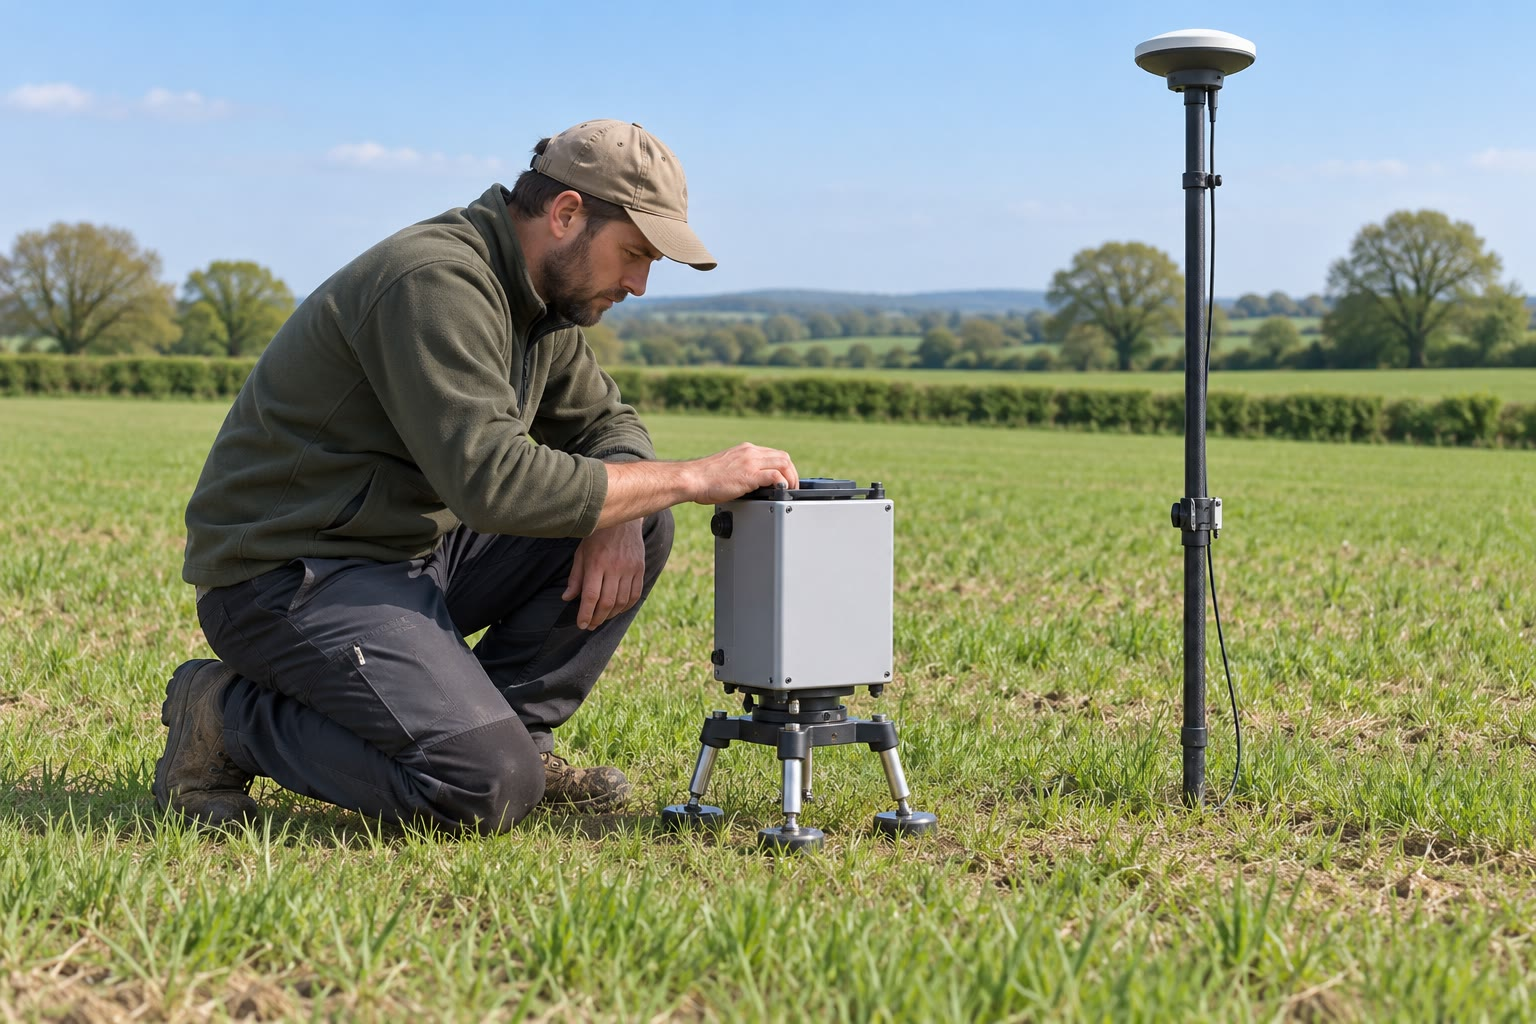
\includegraphics[width=\linewidth]{images/book3/ai/b1-gravity-survey.jpg}

{\scriptsize एक क्षेत्रीय गुरुत्वमापी उसके त्रिपाद पर, उसके बगल में एक उपग्रह-स्थिति एंटीना के साथ (AI से बनाया गया चित्र)।}
\end{minipage}
\end{inthefield}

\section{समस्थिति}

हिमालय के लिए एयरी और प्रैट ने जिस प्रतिपूर्ति की कल्पना की, वह पृथ्वी की बाहरी परतों की एक सामान्य अवस्था का एक उदाहरण है।

\begin{definition}[समस्थिति; प्रतिपूर्ति गहराई]\label{def:b1:isostasy-gravity:isostasy}
किसी क्षेत्र में \emph{समस्थिति}\index{समस्थिति}, अथवा समस्थैतिक साम्य, होता है जब एक गहराई, \emph{प्रतिपूर्ति गहराई}\index{प्रतिपूर्ति गहराई}, विद्यमान हो, जिस पर दाब क्षैतिज सतह के हर बिंदु पर समान हो, ऊपर के उच्चावच चाहे जो हों। प्रतिपूर्ति गहराई के नीचे चट्टानें स्थिर द्रव की तरह व्यवहार करती हैं; उसके ऊपर \omterm{def:b1:layered-earth:layers}{भूपर्पटी} और \omterm{def:b1:layered-earth:layers}{प्रावार} के स्तंभ उन पर तैरते हैं।
\end{definition}

\begin{proposition}[समान द्रव्यमान, प्रतिपूर्ति गहराई के ऊपर]\label{prop:b1:isostasy-gravity:equal-mass}
यदि गुरुत्व $g$ सभी स्तंभों के साथ समान है, तो एक क्षेत्र \omterm{def:b1:isostasy-gravity:isostasy}{प्रतिपूर्ति गहराई} $z_c$ के साथ \omterm{def:b1:isostasy-gravity:isostasy}{समस्थिति} में है यदि और केवल यदि एकाई अनुप्रस्थ-काट का हर ऊर्ध्वाधर स्तंभ, सतह से लेकर $z_c$ तक, एक ही द्रव्यमान रखता है।
\end{proposition}

\begin{proof}
प्रत्येक स्तंभ में चट्टानें द्रवस्थैतिक साम्य में हैं, अतः $\mathrm dp/\mathrm dz = \rho(z)\,g$, जहाँ गहराई $z$ नीचे की ओर गिनी जाती है। सतह पर दाब वायुमंडलीय है, हर जगह एक समान (और नगण्य)। स्तंभ की सतह $z_s$ से $z_c$ तक समाकलित करने पर देता है:
\[
  p(z_c) = p_0 + g\int_{z_s}^{z_c}\rho(z)\,\mathrm dz ,
\]
जहाँ समाकल प्रति एकाई क्षेत्रफल स्तंभ का द्रव्यमान है। $z_c$ पर दाब तभी बराबर हैं जब ये द्रव्यमान बराबर हों।
\end{proof}

दो सरल तरीके द्रव्यमानों के वितरण के दो क्लासिकी प्रतिरूप देते हैं (नीचे का चित्र)।

\begin{proposition}[एयरी समस्थिति]\label{prop:b1:isostasy-gravity:airy}
मान लीजिए \omterm{def:b1:layered-earth:layers}{भूपर्पटी} का एक एकसमान घनत्व $\rho_c$ और मोटाई $H$ है जहाँ उसकी सतह समुद्र-तल पर है, $\rho_m > \rho_c$ घनत्व वाले \omterm{def:b1:layered-earth:layers}{प्रावार} के ऊपर। समस्थैतिक साम्य में:
\begin{enumerate}
  \item जहाँ सतह समुद्र-तल से ऊपर ऊँचाई $h$ पर खड़ी है, वहाँ \omterm{def:b1:layered-earth:layers}{भूपर्पटी} के सामान्य \omterm{def:b1:layered-earth:layers}{भूपर्पटी} के नीचे गहराई $r = h\,\rho_c/(\rho_m - \rho_c)$ की एक जड़ है, और मोटाई $H + h + r$ है;
  \item जहाँ सतह समुद्र-तल से गहराई $d$ पर है, घनत्व $\rho_w$ के पानी के नीचे, वहाँ \omterm{def:b1:layered-earth:layers}{भूपर्पटी} का एक प्रति-जड़ है: उसका आधार $r' = d\,(\rho_c - \rho_w)/(\rho_m - \rho_c)$ से ऊपर उठा है, और उसकी मोटाई $H - d - r'$ है।
\end{enumerate}
यह \emph{एयरी समस्थिति}\index{एयरी समस्थिति} है: घनत्व स्थिर रहते हुए मोटाई के परिवर्तन से प्रतिपूर्ति।
\end{proposition}

\begin{proof}
सबसे गहरी जड़ के ठीक नीचे \omterm{def:b1:isostasy-gravity:isostasy}{प्रतिपूर्ति गहराई} लीजिए, और हर स्तंभ की तुलना सामान्य स्तंभ से कीजिए। (1) ऊँचा स्तंभ गहराई $r$ पर \omterm{def:b1:layered-earth:layers}{प्रावार} की जगह \omterm{def:b1:layered-earth:layers}{भूपर्पटी} रखता है, और ऊँचाई $h$ पर \omterm{def:b1:layered-earth:layers}{भूपर्पटी} रखता है जहाँ सामान्य स्तंभ में कुछ नहीं है: समान द्रव्यमान के लिए $\rho_c(h + r) = \rho_m r$ चाहिए, अर्थात् $r(\rho_m - \rho_c) = \rho_c h$। (2) नीचा स्तंभ गहराई $d$ पर \omterm{def:b1:layered-earth:layers}{भूपर्पटी} की जगह पानी रखता है, और $r'$ पर \omterm{def:b1:layered-earth:layers}{भूपर्पटी} की जगह \omterm{def:b1:layered-earth:layers}{प्रावार}: समान द्रव्यमान के लिए $\rho_w d + \rho_m r' = \rho_c(d + r')$ चाहिए, अर्थात् $r'(\rho_m - \rho_c) =
d(\rho_c - \rho_w)$।
\end{proof}

\begin{proposition}[प्रैट समस्थिति]\label{prop:b1:isostasy-gravity:pratt}
हर स्तंभ समुद्र-तल से नीचे एक ही \omterm{def:b1:isostasy-gravity:isostasy}{प्रतिपूर्ति गहराई} $D$ पर समाप्त हो, हर स्तंभ में एकसमान घनत्व के साथ, जो सतह के समुद्र-तल पर होने पर $\rho_0$ है। समस्थैतिक साम्य में जिस स्तंभ की सतह ऊँचाई $h$ पर खड़ी है, उसका घनत्व है
\[
  \rho(h) = \rho_0\,\frac{D}{D + h},
\]
और पानी की गहराई $d$ के नीचे एक स्तंभ का घनत्व है $\rho = (\rho_0 D - \rho_w d)/(D - d)$। यह \emph{प्रैट समस्थिति}\index{प्रैट समस्थिति} है: स्थिर गहराई पर घनत्व के परिवर्तन से प्रतिपूर्ति।
\end{proposition}

\begin{proof}
$D$ के ऊपर समान द्रव्यमान: ऊँचे स्तंभ के लिए $\rho(h)(D + h) = \rho_0 D$, और नीचे वाले के लिए $\rho_w d + \rho(D - d) = \rho_0 D$।
\end{proof}

$\rho_c = \qty{2700}{kg.m^{-3}}$ और $\rho_m = \qty{3300}{kg.m^{-3}}$ के साथ, एयरी का मूल $h\times2700/600 = 4.5\,h$ है: \qty{2}{km} ऊँची एक श्रेणी का मूल \qty{9}{km} का है, \qty{4}{km} ऊँचे एक पठार का \qty{18}{km}। प्रैट के प्रतिरूप में $D = \qty{100}{km}$ और $\rho_0 = \qty{2700}{kg.m^{-3}}$ के साथ, वही दो स्तंभों के घनत्व 2647 और \qty{2596}{kg.m^{-3}} हैं, दो और चार प्रतिशत हल्के। दोनों प्रतिरूप वही द्रव्यमान संतुलित करते हैं; वे इसमें भिन्न हैं कि हल्की चट्टान कहाँ है, और यह भूकंप-विज्ञान देख सकता है: एयरी पर्वतों के नीचे गहराते \omterm{def:b1:layered-earth:discontinuity}{मोहो} की भविष्यवाणी करता है, प्रैट एक समतल \omterm{def:b1:layered-earth:discontinuity}{मोहो} की।

\begin{omfigure}
\begin{tikzpicture}[x=0.55cm, y=0.05cm, font=\scriptsize]
% columns computed in calc/ch11.py: Airy roots 9 and 18 km, Pratt densities 2647 and 2596 kg/m3;
% heights above sea level drawn five times larger than depths
\begin{scope}
  \node[font=\small] at (4.5,30) {(क) एयरी};
  \fill[omLithGranite!45] (0,0) rectangle (3,-35);
  \fill[omLithGranite!45] (3,10) rectangle (6,-44);
  \fill[omLithGranite!45] (6,20) rectangle (9,-53);
  \fill[omLithPeridotite!45] (0,-35) rectangle (3,-60);
  \fill[omLithPeridotite!45] (3,-44) rectangle (6,-60);
  \fill[omLithPeridotite!45] (6,-53) rectangle (9,-60);
  \draw (0,-60) -- (0,0) -- (3,0) -- (3,10) -- (6,10) -- (6,20) -- (9,20) -- (9,-60);
  \draw (3,0) -- (3,-60) (6,10) -- (6,-60);
  \draw[thick] (0,-35) -- (3,-35) -- (3,-44) -- (6,-44) -- (6,-53) -- (9,-53);
  \draw[densely dashed] (-0.3,-60) -- (9.3,-60);
  \draw[black!50, densely dotted] (-0.3,0) -- (0,0);
  \node[anchor=east] at (-0.3,0) {समुद्र-तल};
  \node[anchor=east] at (-0.3,-35) {35};
  \node[anchor=east] at (-0.3,-60) {60 km};
  \node at (1.5,-17) {2700}; \node at (4.5,-20) {2700}; \node at (7.5,-24) {2700};
  \node at (1.5,-50) {3300};
  \node[anchor=south] at (1.5,0) {$h = 0$};
  \node[anchor=south] at (4.5,10) {$h = 2$};
  \node[anchor=south] at (7.5,20) {$h = 4$};
  \draw[black!45, densely dotted] (3,-35) -- (9,-35);
  \node at (4.5,-39.5) {मूल 9};
  \node at (7.5,-44) {मूल 18};
\end{scope}
\begin{scope}[xshift=7.9cm]
  \node[font=\small] at (4.5,30) {(ख) प्रैट};
  \fill[omLithGranite!45] (0,0) rectangle (3,-100);
  \fill[omLithGranite!36] (3,10) rectangle (6,-100);
  \fill[omLithGranite!27] (6,20) rectangle (9,-100);
  \draw (0,-100) -- (0,0) -- (3,0) -- (3,10) -- (6,10) -- (6,20) -- (9,20) -- (9,-100);
  \draw (3,0) -- (3,-100) (6,10) -- (6,-100);
  \draw[densely dashed] (-0.3,-100) -- (9.3,-100);
  \draw[black!50, densely dotted] (-0.3,0) -- (0,0);
  \node[anchor=east] at (-0.3,0) {समुद्र-तल};
  \node[anchor=east] at (-0.3,-100) {$D = 100$ km};
  \node at (1.5,-50) {2700}; \node at (4.5,-50) {2647}; \node at (7.5,-50) {2596};
  \node[anchor=south] at (1.5,0) {$h = 0$};
  \node[anchor=south] at (4.5,10) {$h = 2$};
  \node[anchor=south] at (7.5,20) {$h = 4$};
\end{scope}
\end{tikzpicture}

\par\smallskip{\small \omterm{def:b1:isostasy-gravity:isostasy}{समस्थिति} के दो क्लासिकी प्रतिरूप, तीन स्तंभों के लिए जो समुद्र-तल से 0, 2 और \qty{4}{km} ऊपर खड़े हैं (ऊँचाइयाँ गहराइयों से पाँच गुना बढ़ाकर दिखाई गई हैं; घनत्व \unit{kg.m^{-3}} में)। (क) एयरी: \omterm{def:b1:layered-earth:layers}{भूपर्पटी} का एक घनत्व, ऊँचाई का 4.5 गुना मूल। (ख) प्रैट: एक \omterm{def:b1:isostasy-gravity:isostasy}{प्रतिपूर्ति गहराई}, ऊँची भूमि के नीचे हल्के स्तंभ। हर स्तंभ ऊपर के बिंदुकित \omterm{def:b1:isostasy-gravity:isostasy}{प्रतिपूर्ति गहराई} के ऊपर प्रति एकाई क्षेत्रफल एक ही द्रव्यमान रखता है।}
\label{fig:b1:isostasy-gravity:models}
\end{omfigure}

\omterm{def:b1:isostasy-gravity:isostasy}{समस्थिति} एक ऐसा कथन है जो लंबे समयों में विस्तृत क्षेत्रों के बारे में है। \omterm{def:b1:layered-earth:lithosphere}{दुर्बलमंडल} केवल उन भारों के आगे झुकता है जो हज़ारों वर्षों तक बने रहते हैं, और उसके ऊपर का \omterm{def:b1:layered-earth:lithosphere}{स्थलमंडल} इतना कठोर है कि एक संकीर्ण भार को मोड़कर एक व्यापक क्षेत्र पर फैला दे, जैसे एक तख़्ता भार उठाता है: एक अकेला ज्वालामुखी अपने ही नीचे प्रतिपूर्ति नहीं पाता; \omterm{def:b1:layered-earth:lithosphere}{स्थलमंडल} का यह मोड़ पुस्तक 5 में पढ़ा जाता है। बड़ी पर्वत-शृंखलाओं के नीचे \omterm{def:b1:layered-earth:layers}{भूपर्पटी} उसके महाद्वीपीय औसत, लगभग \qty{30}{km} से कहीं अधिक मोटी है: एयरी का चित्र, हल्की \omterm{def:b1:layered-earth:layers}{भूपर्पटी} की जड़ें, पर्वत-शृंखलाओं के लिए अधिक निकट है। प्रैट का, स्थिर गहराई पर हल्की चट्टान, मध्य-महासागरीय कटकों की व्याख्या करता है, जो एक ऊपरी \omterm{def:b1:layered-earth:layers}{प्रावार} के ऊपर ऊँचे खड़े रहते हैं जिसे उसके ऊँचे तापमान ने हल्का कर दिया है।
% ledger: usgs:crust-thickness

\subsection*{पृथ्वी के दो स्तर}

\omterm{def:b1:isostasy-gravity:isostasy}{समस्थिति} पूरे ग्रह के उच्चावच को व्यवस्थित करती है। उसका वितरण एक वक्र से सारांशित होता है।

\begin{definition}[हिप्सोमेट्रिक वक्र]\label{def:b1:isostasy-gravity:hypsometry}
किसी ग्रह का \emph{हिप्सोमेट्रिक वक्र}\index{हिप्सोमेट्रिक वक्र} उसकी सतह के हर अंश $f$ के लिए वह उन्नयन $z(f)$ देता है, जिसे ठीक उतना ही अंश पार करता है। यह ऊपर से पढ़े गए उन्नयन का संचयी वितरण है।
\end{definition}

इसे एक ग्रिड वाले उन्नयन-प्रतिरूप से खींचने के लिए हर ग्रिड-कोष्ठक को उसके क्षेत्रफल से भारित करना होगा। \omterm{def:b1:spherical-astronomy:geographic}{अक्षांश} और \omterm{def:b1:spherical-astronomy:geographic}{देशांतर} में एक-एक डिग्री के ग्रिड पर, अक्षांशों $\varphi_1$ और $\varphi_2$ के बीच का कोष्ठक क्षेत्रफल $R^2\,\Delta\lambda\,(\sin\varphi_2 - \sin\varphi_1)$ रखता है, जो ध्रुवों की ओर सिकुड़ता है; सभी कोष्ठकों पर जोड़ने से क्षेत्रफल ठीक $4\pi R^2$ देते हैं। कोष्ठकों को उन्नयन के अनुसार छाँटकर और उनके क्षेत्रफल संचित करके नीचे के चित्र का वक्र मिलता है। वह दिखाता है कि सतह का \qty{70.9}{\percent} भाग समुद्र-तल से नीचे है; कि भूमि का औसत उन्नयन लगभग \qty{0.8}{km} है और महासागर की औसत गहराई लगभग \qty{3.7}{km}; और कि सतह का अधिकांश भाग दो सपाट सोपानों में से एक का है, समुद्र-तल के निकट महाद्वीपीय मंच और लगभग 3.5 से \qty{6}{km} नीचे का अतल तल, जो एक तीखी ढलान से जुड़े हैं।
% computed in figdata/bachelor-1/hypsometry.py (fraction 0.709, land 793 m, ocean 3692 m); ledger: data:etopo1, wss:ocean-cover

एक ग्रह जिसकी एक ही प्रकार की \omterm{def:b1:layered-earth:layers}{भूपर्पटी} हो, जिसका उच्चावच यादृच्छिक रूप से उठा और घिसा हो, एक ही स्तर रखता, जिसके चारों ओर उन्नयन बिखरे होते। पृथ्वी के दो हैं, क्योंकि उसकी समस्थैतिक साम्य में दो प्रकार की \omterm{def:b1:layered-earth:layers}{भूपर्पटी} है: मोटी, हल्की महाद्वीपीय \omterm{def:b1:layered-earth:layers}{भूपर्पटी} ऊँची तैरती है, पतली, सघन महासागरीय \omterm{def:b1:layered-earth:layers}{भूपर्पटी} नीची (पुस्तक 2, कक्षा 11)। \Cref{exo:b1:isostasy-gravity:8} दिखाता है कि एयरी का एक भूपर्पटी-घनत्व वाला प्रतिरूप प्रेक्षित भूपर्पटी-मोटाइयों के साथ दोनों स्तर उत्पन्न नहीं कर सकता।

\begin{omfigure}
\begin{tikzpicture}
\begin{axis}[omrecord, width=0.84\linewidth, height=6.4cm, xmin=0, xmax=100, ymin=-11, ymax=9,
  xlabel={पृथ्वी की सतह का वह अंश जो ऊँचा है (\unit{\percent})},
  ylabel={उन्नयन (km)}, xtick={0,10,...,100}, ytick={-10,-8,...,8},
  tick label style={font=\scriptsize}, label style={font=\small}, clip=true]
% computed in figdata/bachelor-1/hypsometry.py; ledger: data:etopo1
\addplot[name path=hyps, very thick, black] table[x=area_pc, y expr=\thisrow{elev}/1000] {figdata/out/bachelor-1-hypsometry-curve.dat};
\path[name path=sea] (axis cs:0,0) -- (axis cs:100,0);
\addplot[omSea!60] fill between[of=hyps and sea, soft clip={domain=29.1:100}];
\addplot[omHypsLandC!80] fill between[of=hyps and sea, soft clip={domain=0:29.1}];
\draw[black!60, densely dotted] (axis cs:0,0) -- (axis cs:100,0);
\draw[black!60, densely dashed] (axis cs:29.1,-11) -- (axis cs:29.1,9);
\draw[omSea!60!black, densely dashed] (axis cs:29.1,-3.692) -- (axis cs:100,-3.692);
\draw[omHypsLandF, densely dashed] (axis cs:0,0.793) -- (axis cs:29.1,0.793);
  \node[font=\scriptsize, anchor=south east] at (axis cs:99,0.1) {समुद्र-तल};
  \node[font=\scriptsize, anchor=south, align=center] at (axis cs:18,1.0) {भूमि का औसत\\उन्नयन \qty{0.79}{km}};
  \node[font=\scriptsize, anchor=north west, align=left] at (axis cs:31,-3.9) {महासागर की औसत\\गहराई \qty{3.69}{km}};
  \node[font=\scriptsize, anchor=north west, align=left] at (axis cs:30.5,6.5) {भूमि: \qty{29.1}{\percent}\\सतह का};
  \node[font=\scriptsize, anchor=north, align=center] at (axis cs:17,-0.5) {महाद्वीपीय\\मंच};
  \node[font=\scriptsize] at (axis cs:62,-5.2) {अतल तल};
\end{axis}
\end{tikzpicture}

\par\smallskip{\small पृथ्वी का \omterm{def:b1:isostasy-gravity:hypsometry}{हिप्सोमेट्रिक वक्र}, एक डिग्री पर ETOPO1 वैश्विक उच्चावच-प्रतिरूप से, हर कोष्ठक उसके क्षेत्रफल से भारित (अंटार्कटिका और ग्रीनलैंड पर, बर्फ़ का ऊपरी सिरा)। वक्र के दो लगभग सपाट खंड समुद्र-तल के निकट महाद्वीपीय मंच और गहरे महासागरीय तल हैं।}
\label{fig:b1:isostasy-gravity:hypsometry}
\end{omfigure}

\section{गुरुत्व विसंगतियाँ}

\subsection*{दो सुधार}

पहाड़ी पर का गुरुत्वमापी पृथ्वी के केंद्र से समुद्र-तल वाले की तुलना में अधिक दूर है, और चट्टान की एक ऐसी परत पर खड़ा है जो दूसरे के नीचे नहीं है। दोनों प्रभाव माप की \omterm{def:b1:isostasy-gravity:normal-gravity}{सामान्य गुरुत्व} से तुलना से पहले परिकलित किए जाते हैं।

\begin{proposition}[मुक्त-वायु प्रवणता]\label{prop:b1:isostasy-gravity:free-air}
त्रिज्या $R$ के एक गोलीय पृथ्वी के बाहर, गुरुत्व ऊँचाई $h$ के साथ इस दर से घटता है:
\[
  \frac{\mathrm dg}{\mathrm dh} = -\frac{2g}{R}\,;
\]
सतह पर, $2g/R \approx \qty{3.08e-6}{s^{-2}}$, लगभग \qty{0.308}{\milli\gal} प्रति मीटर।
\end{proposition}

\begin{proof}
$g(r) = GM/r^2$, अतः $\mathrm dg/\mathrm dr = -2GM/r^3 = -2g(r)/r$; $r = R$ पर, साथ में $g = \qty{9.820}{m.s^{-2}}$ और $R = \qty{6371}{km}$, $2g/R =
\qty{3.083e-6}{s^{-2}}$।
\end{proof}
% ledger: earth:gmean, earth:Rmean

समतलीकरण और घूर्णन प्रवणता को थोड़ा बदलते हैं; व्यवहार में प्रयुक्त मान \qty{0.3086}{\milli\gal.m^{-1}} है।
% ledger: usgs73:reduction

\begin{proposition}[बूगेर पट्टी]\label{prop:b1:isostasy-gravity:slab}
मोटाई $h$ और एकसमान घनत्व $\rho$ की एक अनंत क्षैतिज पट्टी उसके बाहर के एक बिंदु को ऊर्ध्वाधर त्वरण के साथ आकर्षित करती है:
\[
  g_B = 2\pi G\rho h ,
\]
बिंदु से पट्टी तक की दूरी चाहे जो हो। संख्यात्मक रूप से $2\pi G =
\qty{0.0419}{\milli\gal}$ प्रति मीटर मोटाई और प्रति \qty{1000}{kg.m^{-3}} घनत्व पर।
\end{proposition}

\begin{proof}
बिंदु को मूलबिंदु पर रखिए और पट्टी को उसके आरपार ऊर्ध्वाधर के समाक्षीय पतले वलयों में काटिए। बिंदु के नीचे दूरी $z$ पर, त्रिज्या $s$, चौड़ाई $\mathrm ds$ और मोटाई $\mathrm dz$ का एक वलय, द्रव्यमान $\rho\,2\pi s\,\mathrm ds\,\mathrm dz$ रखता है, सब दूरी $\sqrt{s^2 + z^2}$ पर; समरूपता से उसका आकर्षण ऊर्ध्वाधर है, हर तत्व के आकर्षण का उसके ऊर्ध्वाधर से कोण के कोसाइन $z/\sqrt{s^2+z^2}$ गुना:
\[
  \mathrm dg = G\,\frac{\rho\,2\pi s\,\mathrm ds\,\mathrm dz}{s^2 + z^2}\,
  \frac{z}{\sqrt{s^2 + z^2}} .
\]
एक परत के लिए, $\int_0^\infty s\,(s^2 + z^2)^{-3/2}\,\mathrm ds =
\bigl[-(s^2 + z^2)^{-1/2}\bigr]_0^\infty = 1/z$ है, अतः परत $2\pi G\rho\,\mathrm dz$ के साथ आकर्षित करती है, जो $z$ से स्वतंत्र है। मोटाई $h$ पर परतों को जोड़ने से $2\pi G\rho h$ मिलता है। $G = \qty{6.674e-11}{m^3.kg^{-1}.s^{-2}}$ के साथ, $2\pi G\times\qty{1000}{kg.m^{-3}}\times\qty{1}{m} = \qty{4.19e-7}{m.s^{-2}} =
\qty{0.0419}{\milli\gal}$।
\end{proof}
% ledger: const:G

\begin{definition}[गुरुत्व विसंगतियाँ]\label{def:b1:isostasy-gravity:anomalies}
मान लीजिए $g$ \omterm{def:b1:spherical-astronomy:geographic}{अक्षांश} $\varphi$ और समुद्र-तल से ऊँचाई $h$ पर एक स्टेशन पर मापा गया गुरुत्व है।
\begin{itemize}
  \item एक \emph{गुरुत्व विसंगति}\index{गुरुत्व विसंगति} एक सामान्य स्तर तक सुधारे गए मापित गुरुत्व और उसी \omterm{def:b1:spherical-astronomy:geographic}{अक्षांश} पर \omterm{def:b1:isostasy-gravity:normal-gravity}{सामान्य गुरुत्व} के बीच का अंतर है।
  \item \emph{मुक्त-वायु सुधार}\index{मुक्त-वायु सुधार} है $+\qty{0.3086}{\milli\gal.m^{-1}}\times h$: यह गुरुत्व की ऊँचाई के साथ कमी को वापस जोड़ता है। \emph{मुक्त-वायु विसंगति}\index{मुक्त-वायु विसंगति} है $\Delta g_{\mathrm{FA}} = g + 0.3086\,h - \gamma(\varphi)$।
  \item \emph{बूगेर सुधार}\index{बूगेर सुधार} है $-2\pi G\rho h$: यह स्टेशन और समुद्र-तल के बीच की चट्टान का आकर्षण हटाता है, जिसे घनत्व $\rho$ की एक पट्टी माना जाता है, परंपरागत रूप से \qty{2670}{kg.m^{-3}}, जो प्रति मीटर \qty{0.112}{\milli\gal} देता है। \emph{बूगेर विसंगति}\index{बूगेर विसंगति} है $\Delta g_{\mathrm B} = \Delta g_{\mathrm{FA}} - 2\pi G\rho h$।
\end{itemize}
\end{definition}
% ledger: usgs73:reduction, swisstopo:bouguer-map

पट्टी खुरदुरे देश में एक स्टेशन के चारों ओर की भूमि का एक मोटा प्रतिरूप है: स्टेशन के नीचे की घाटियाँ उस चट्टान के रूप में गिनी जाती हैं जो वहाँ नहीं है, और उसके ऊपर की पहाड़ियाँ ऊपर खींचती हैं और बिल्कुल नहीं गिनी जातीं। एक तीसरा अपचयन, भूभाग सुधार, जो एक अंकीय उन्नयन-प्रतिरूप से परिकलित होता है, दोनों त्रुटियाँ हटाता है। समुद्र पर \omterm{def:b1:isostasy-gravity:anomalies}{मुक्त-वायु सुधार} शून्य होता है, और बूगेर अपचयन पानी की जगह चट्टान रखता है।

\begin{method}[गुरुत्व-पाठ का अपचयन]\label{met:b1:isostasy-gravity:reduction}
\begin{enumerate}
  \item स्टेशन के \omterm{def:b1:spherical-astronomy:geographic}{अक्षांश} पर \omterm{def:b1:isostasy-gravity:normal-gravity}{सामान्य गुरुत्व} $\gamma(\varphi)$ परिकलित कीजिए।
  \item मापे गए गुरुत्व में \omterm{def:b1:isostasy-gravity:anomalies}{मुक्त-वायु सुधार} $0.3086\,h$ (\unit{\milli\gal} में, $h$ मीटर में) जोड़िए और $\gamma$ घटाइए: यह \omterm{def:b1:isostasy-gravity:anomalies}{मुक्त-वायु विसंगति} है।
  \item \omterm{def:b1:isostasy-gravity:anomalies}{बूगेर सुधार} $0.0419\times(\rho/1000)\times h$ घटाइए, जो मानक घनत्व के लिए $0.112\,h$ है: यह \omterm{def:b1:isostasy-gravity:anomalies}{बूगेर विसंगति} है।
  \item पूरे हिसाब में मिलीगैल में काम कीजिए, और मापे गए तथा \omterm{def:b1:isostasy-gravity:normal-gravity}{सामान्य गुरुत्व} को सात सार्थक अंकों तक रखिए: विसंगति दो बड़ी संख्याओं का एक छोटा अंतर है।
\end{enumerate}
\end{method}

\begin{example}[एक पहाड़ी पर स्टेशन]\label{ex:b1:isostasy-gravity:reduction}
समुद्र-तल से \qty{1200}{m} ऊपर और \ang{45} \omterm{def:b1:spherical-astronomy:geographic}{अक्षांश} के एक स्टेशन पर गुरुत्वमापी \qty{9.802597}{m.s^{-2}} देता है। वहाँ का \omterm{def:b1:isostasy-gravity:normal-gravity}{सामान्य गुरुत्व} \qty{9.806200}{m.s^{-2}} है; मापा गया मान \qty{360.3}{\milli\gal} कम है। \omterm{def:b1:isostasy-gravity:anomalies}{मुक्त-वायु सुधार} $0.3086\times1200 = \qty{370.3}{\milli\gal}$ है, अतः $\Delta g_{\mathrm{FA}} = -360.3 + 370.3 = \qty{+10.0}{\milli\gal}$। \omterm{def:b1:isostasy-gravity:anomalies}{बूगेर सुधार} $0.112\times1200 = \qty{134.4}{\milli\gal}$ है, अतः $\Delta g_{\mathrm B}
= \qty{-124.4}{\milli\gal}$: समुद्र-तल से ऊपर की चट्टान हटाने के बाद इस स्टेशन के नीचे समुद्र-तल वाले स्टेशन के नीचे की तुलना में कम द्रव्यमान है।
\end{example}

\subsection*{विसंगतियाँ प्रतिपूर्ति के बारे में क्या कहती हैं}

\begin{proposition}[व्यापक उच्चावच पर विसंगतियाँ]\label{prop:b1:isostasy-gravity:broad}
मान लीजिए ऊँचाई $h$ और घनत्व $\rho_c$ का एक पठार है, जो अपनी \omterm{def:b1:isostasy-gravity:isostasy}{प्रतिपूर्ति गहराई} से कहीं अधिक चौड़ा है, और उसके केंद्र के निकट एक स्टेशन। बूगेर घनत्व को $\rho_c$ के बराबर लीजिए।
\begin{enumerate}
  \item यदि पठार प्रतिपूर्ति नहीं है, तो $\Delta g_{\mathrm{FA}} \approx
        2\pi G\rho_c h$ और $\Delta g_{\mathrm B} \approx 0$।
  \item यदि वह समस्थैतिक साम्य में है, प्रतिपूर्ति करने वाले द्रव्यमानों का वितरण चाहे जो हो, $\Delta g_{\mathrm{FA}} \approx 0$ और
        $\Delta g_{\mathrm B} \approx -2\pi G\rho_c h$।
\end{enumerate}
\end{proposition}

\begin{proof}
स्टेशन की ऊँचाई पर \omterm{def:b1:isostasy-gravity:normal-gravity}{सामान्य गुरुत्व} $\gamma - 0.3086\,h$ है, अतः \omterm{def:b1:isostasy-gravity:anomalies}{मुक्त-वायु विसंगति} सामान्य स्तंभ से भिन्न द्रव्यमानों का आकर्षण है। एक चौड़े पठार के केंद्र के निकट इन असामान्य द्रव्यमानों की हर परत एक अनंत पट्टी की तरह कार्य करती है, और \cref{prop:b1:isostasy-gravity:slab} से घनत्व-अंतर $\Delta\rho$ और मोटाई $t$ की एक पट्टी, जहाँ भी वह हो, $2\pi G\Delta\rho
t$ से आकर्षित करती है। कुल, प्रति एकाई क्षेत्रफल असामान्य द्रव्यमान का $2\pi G$ गुना है। (1) प्रतिपूर्ति के बिना वह द्रव्यमान $\rho_c h$ है। (2) \omterm{def:b1:isostasy-gravity:isostasy}{समस्थिति} में, \cref{prop:b1:isostasy-gravity:equal-mass} से, वह शून्य है। दोनों स्थितियों में \omterm{def:b1:isostasy-gravity:anomalies}{बूगेर सुधार} $2\pi G\rho_c h$ घटाता है।
\end{proof}

एयरी प्रतिपूर्ति के लिए दूसरी स्थिति का \omterm{def:b1:isostasy-gravity:anomalies}{बूगेर विसंगति} भी $-2\pi G(\rho_m - \rho_c)r$ है, मूल के लुप्त द्रव्यमान का आकर्षण, क्योंकि $(\rho_m - \rho_c)r = \rho_c h$। विस्तृत क्षेत्रों पर शून्य के निकट मुक्त-वायु विसंगतियाँ इस प्रकार \omterm{def:b1:isostasy-gravity:isostasy}{समस्थिति} का चिह्न हैं, और बूगेर विसंगतियाँ जो उच्चावच का दर्पण-प्रतिबिंब अनुसरण करती हैं, प्रतिपूर्ति करने वाले द्रव्यमानों को मापती हैं: बूगेर विसंगतियाँ आल्प्स के पूरे विस्तार में क्षेत्रीय रूप से ऋणात्मक हैं, और मध्य-महासागरीय कटकों पर, वे चाहे जितने ऊँचे हों, \omterm{def:b1:isostasy-gravity:anomalies}{मुक्त-वायु विसंगति} छोटी है। महासागरों पर \omterm{def:b1:isostasy-gravity:anomalies}{बूगेर विसंगति} धनात्मक है: पानी की जगह चट्टान रखने से उस स्तंभ पर द्रव्यमान जुड़ता है जिससे कोई द्रव्यमान गायब नहीं है।
% ledger: swisstopo:bouguer-map

उच्चावच के किनारों के निकट पट्टी का सन्निकटन विफल होता है, क्योंकि उच्चावच स्टेशन के निकट है और मूल उसके नीचे बहुत दूर। नीचे का चित्र एक प्रतिरूप श्रेणी, जो \qty{200}{km} चौड़ी और \qty{2}{km} ऊँची है, का सटीक आकर्षण देता है। प्रतिपूर्ति के बिना, \omterm{def:b1:isostasy-gravity:anomalies}{मुक्त-वायु विसंगति} केंद्र पर \qty{+225}{\milli\gal} है, जो पट्टी के मान \qty{226}{\milli\gal} के निकट है; \qty{9}{km} के एयरी मूल के साथ, केंद्र की \omterm{def:b1:isostasy-gravity:anomalies}{मुक्त-वायु विसंगति} \qty{+55}{\milli\gal} तक गिरती है, शून्य तक नहीं, क्योंकि केवल \qty{200}{km} चौड़ी श्रेणी अपने मूल से \qty{40}{km} ऊपर से अनंत नहीं दिखती, और \omterm{def:b1:isostasy-gravity:anomalies}{मुक्त-वायु विसंगति} हर किनारे के ठीक बाहर तीखी ऋणात्मक हो जाती है, जहाँ स्टेशन मूल देखता है पर पर्वत नहीं।
% computed in figdata/bachelor-1/gravity_profiles.py (centre values 225.0, -1.4, 55.2, -171.2 mGal)

\begin{omfigure}
\begin{tikzpicture}
\begin{axis}[omrecord, name=anom, width=0.86\linewidth, height=6.2cm, xmin=-300, xmax=300, ymin=-310, ymax=250,
  ylabel={विसंगति (\unit{\milli\gal})}, xticklabels={}, ytick={-200,-100,0,100,200},
  tick label style={font=\scriptsize}, label style={font=\small},
  legend style={font=\scriptsize, at={(0.01,0.01)}, anchor=south west, draw=none, fill=white, fill opacity=0.85, text opacity=1},
  legend cell align=left, legend columns=2]
% computed in figdata/bachelor-1/gravity_profiles.py
\addplot[very thick, red!75!black] table[x=x, y=fa_unc] {figdata/out/bachelor-1-gravity_profiles-profiles.dat};
\addlegendentry{मुक्त-वायु, अप्रतिपूरित}
\addplot[thick, red!75!black, densely dashed] table[x=x, y=bg_unc] {figdata/out/bachelor-1-gravity_profiles-profiles.dat};
\addlegendentry{बूगेर, अप्रतिपूरित}
\addplot[very thick, blue!70!black] table[x=x, y=fa_airy] {figdata/out/bachelor-1-gravity_profiles-profiles.dat};
\addlegendentry{मुक्त-वायु, एयरी मूल}
\addplot[thick, blue!70!black, densely dashed] table[x=x, y=bg_airy] {figdata/out/bachelor-1-gravity_profiles-profiles.dat};
\addlegendentry{बूगेर, एयरी मूल}
\draw[black!50, densely dotted] (axis cs:-300,0) -- (axis cs:300,0);
\end{axis}
\begin{axis}[at={(anom.south west)}, anchor=north west, yshift=-0.25cm, width=0.86\linewidth, height=3.6cm,
  xmin=-300, xmax=300, ymin=-50, ymax=5, axis background/.style={fill=white},
  xlabel={श्रेणी के केंद्र से दूरी (km)}, ylabel={गहराई (km)},
  ytick={0,-35,-44}, yticklabels={0,35,44}, tick label style={font=\scriptsize}, label style={font=\small}]
\fill[omLithPeridotite!45] (axis cs:-300,-50) rectangle (axis cs:300,-35);
\fill[omLithGranite!45] (axis cs:-300,-35) rectangle (axis cs:300,0);
\fill[omLithGranite!45] (axis cs:-100,0) rectangle (axis cs:100,2);
\fill[omLithGranite!45, pattern color=blue!60!black, postaction={pattern=north east lines, pattern color=blue!50!black}] (axis cs:-100,-35) rectangle (axis cs:100,-44);
\draw (axis cs:-300,0) -- (axis cs:-100,0) -- (axis cs:-100,2) -- (axis cs:100,2) -- (axis cs:100,0) -- (axis cs:300,0);
\draw[thick] (axis cs:-300,-35) -- (axis cs:300,-35);
\draw[thick, blue!60!black] (axis cs:-100,-35) -- (axis cs:-100,-44) -- (axis cs:100,-44) -- (axis cs:100,-35);
\node[font=\scriptsize] at (axis cs:-200,-17) {भूपर्पटी 2700};
\node[font=\scriptsize] at (axis cs:-200,-43) {प्रावार 3300};
\node[font=\scriptsize, fill=white, inner sep=1pt, anchor=west] at (axis cs:105,-40) {एयरी मूल (दूसरा प्रतिरूप)};
\node[font=\scriptsize, anchor=south] at (axis cs:0,2) {श्रेणी, \qty{2}{km} ऊँची};
\end{axis}
\end{tikzpicture}

\par\smallskip{\small ऊपर: एक प्रतिरूप श्रेणी के आरपार मुक्त-वायु और बूगेर विसंगतियाँ, जो \qty{200}{km} चौड़ी और \qty{2}{km} ऊँची है, द्विविमीय पिंडों के लिए सटीक परिकलित, ज़मीनी सतह पर स्टेशनों के साथ (कोई भूभाग सुधार नहीं)। नीचे: प्रतिरूप (ऊर्ध्वाधर पैमाना दो गुने से कम बढ़ाया गया); मूल केवल प्रतिपूरित स्थिति में विद्यमान है। अप्रतिपूरित, \omterm{def:b1:isostasy-gravity:anomalies}{मुक्त-वायु विसंगति} उच्चावच का अनुसरण करती है और \omterm{def:b1:isostasy-gravity:anomalies}{बूगेर विसंगति} लगभग शून्य है; प्रतिपूरित, \omterm{def:b1:isostasy-gravity:anomalies}{मुक्त-वायु विसंगति} केंद्र पर छोटी है, तीखे किनारे-प्रभावों के साथ, और \omterm{def:b1:isostasy-gravity:anomalies}{बूगेर विसंगति} एक चौड़ी गर्त है।}
\label{fig:b1:isostasy-gravity:profiles}
\end{omfigure}

\begin{method}[एक क्षेत्र की समस्थिति की जाँच]\label{met:b1:isostasy-gravity:test}
\begin{enumerate}
  \item उच्चावच के किनारों से दूर, \omterm{def:b1:layered-earth:layers}{भूपर्पटी} की मोटाई से कई गुना चौड़े क्षेत्र पर \omterm{def:b1:isostasy-gravity:anomalies}{मुक्त-वायु विसंगति} का औसत लीजिए।
  \item यदि वह शून्य के निकट है, तो क्षेत्र प्रतिपूरित है; यदि वह औसत ऊँचाई के गुणा $2\pi G\rho_c$ के निकट पहुँचती है, तो नहीं।
  \item अनुपात $-\Delta g_{\mathrm B}/(2\pi G\rho_c h)$ उच्चावच का वह अंश देता है जो प्रतिपूरित है।
  \item \omterm{def:b1:layered-earth:discontinuity}{मोहो} की गहराई पर भूकंपीय या अन्य प्रमाण एयरी की प्रतिपूर्ति को प्रैट की से अलग बताते हैं: अकेला विस्तृत गुरुत्व नहीं बता सकता, क्योंकि दोनों उच्चावच के नीचे एक ही द्रव्यमान-कमी रखते हैं।
\end{enumerate}
\end{method}

\begin{history}[समुद्र पर गुरुत्व]
\begin{minipage}[t]{0.58\linewidth}\vspace{0pt}
एक लोलक अपने आवर्तकाल से गुरुत्व मापता है, पर एक जहाज़ पर लहरें उसे किसी भी विसंगति से कहीं अधिक हिलाती हैं। 1920 के दशक में डच भू-मापक फ़ेलिक्स वेनिंग मायनेज़ ने उपाय खोजा: एक ही चौखट में विपरीत कला में झूलते दो लोलक जहाज़ के वही क्षैतिज त्वरण महसूस करते हैं, और उनका अंतर उन्हें निरस्त कर देता है। 1923 से उन्होंने अपना उपकरण डच नौसेना की पनडुब्बियों पर ले जाया, जहाँ डूबे होने पर वह लहरों के सबसे बुरे प्रभाव से बच जाता था, पहले पूर्वी द्वीपसमूह की एक यात्रा पर और फिर उनके समुद्रों के सर्वेक्षणों में। द्वीपसमूह की गहरी समुद्री खाइयों के साथ उन्हें ऋणात्मक समस्थैतिक विसंगतियों की लंबी पट्टियाँ मिलीं, और फिर उन्होंने वे अन्य खाइयों के साथ भी पाईं: वे उन्हें केवल ऐसी \omterm{def:b1:layered-earth:layers}{भूपर्पटी} से समझा सकते थे जिसे वहाँ बाहरी बलों द्वारा नीचे दबाया गया हो, और जो समस्थैतिक साम्य से बाहर हो।
% ledger: egs:vening-meinesz
\end{minipage}\hfill
\begin{minipage}[t]{0.38\linewidth}\vspace{0pt}
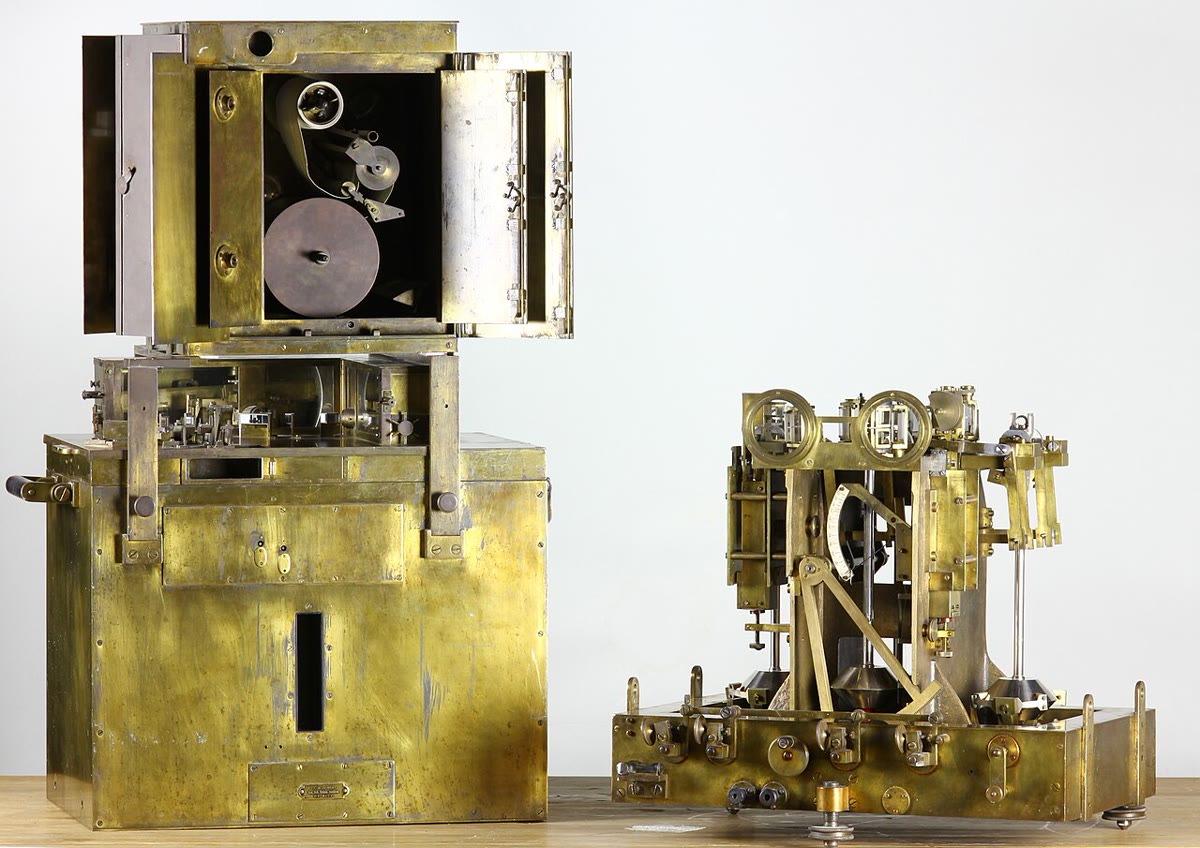
\includegraphics[width=\linewidth]{images/book3/b1-vening-meinesz.jpg}

{\scriptsize एक वेनिंग मायनेज़ लोलक उपकरण (दाएँ) और रिकॉर्डिंग इकाई के साथ उसका डिब्बा (Broodt, CC BY-SA 4.0)।}
\end{minipage}
\end{history}

\section{जियॉइड}

स्थिर समुद्र-सतह स्थिर गुरुत्व-विभव की एक सतह है: यदि ऐसा न होता, तो पानी उस पर बहता। वह ऊँचाइयों के लिए स्वाभाविक संदर्भ है, वह सतह जिस पर पुरानी ओलंब-रेखाएँ लंबवत थीं।

\begin{definition}[जियॉइड; जियॉइड ऊँचाई]\label{def:b1:isostasy-gravity:geoid}
\emph{जियॉइड}\index{जियॉइड} पृथ्वी के गुरुत्व (गुरुत्वाकर्षण और घूर्णन के अपकेंद्री प्रभाव का योग) का वह समविभव पृष्ठ है जो खुले महासागरों पर स्थिर औसत समुद्र-सतह के साथ संपाती है, और महाद्वीपों के नीचे आगे बढ़ाया जाता है। किसी बिंदु पर \emph{जियॉइड ऊँचाई}\index{जियॉइड ऊँचाई} $N$ संदर्भ दीर्घवृत्तज के ऊपर जियॉइड की ऊँचाई है, जहाँ जियॉइड उसके नीचे है वहाँ ऋणात्मक गिनी जाती है।
\end{definition}

मानचित्रों पर समुद्र-तल से ऊपर की ऊँचाइयाँ \omterm{def:b1:isostasy-gravity:geoid}{जियॉइड} से ऊपर की ऊँचाइयाँ हैं; उपग्रह स्थिति-निर्धारण से दी गई ऊँचाइयाँ दीर्घवृत्तज से ऊपर की हैं; दोनों $N$ से भिन्न हैं। \omterm{def:b1:isostasy-gravity:geoid}{जियॉइड} आइसलैंड के निकट \qty{+85}{m} और दक्षिणी भारत के तट पर \qty{-106}{m} दीर्घवृत्तज से हटता है, कुल मिलाकर \qty{200}{m} से कम, जबकि ठोस सतह का उच्चावच लगभग \qty{20}{km} फैला है: \omterm{def:b1:isostasy-gravity:geoid}{जियॉइड} ज़मीन से कहीं अधिक चिकनी सतह है।
% ledger: nasa:geoid-range, earth:topo

\begin{proposition}[जियॉइड ऊँचाई और विभव-विसंगति]\label{prop:b1:isostasy-gravity:bruns}
माना $\Phi$ पृथ्वी का गुरुत्वीय विभव है और $\Phi_n$ सामान्य विभव, उस प्रतिरूप पृथ्वी का जिसकी सतह, संदर्भ दीर्घवृत्तज, का वही विभव $\Phi_0$ है जो \omterm{def:b1:isostasy-gravity:geoid}{जियॉइड} का है; दोनों भौतिकी के चिह्न से गिने गए (विभव ऊपर की ओर बढ़ता है और $g = -\nabla\Phi$)। माना $T = \Phi - \Phi_n$ \omterm{def:b1:isostasy-gravity:geoid}{जियॉइड} पर विभव-विसंगति है। पहली कोटि तक,
\[
  N = -\frac{T}{\gamma} .
\]
भूमितिज्ञ, जो विभव को विपरीत चिह्न से गिनते हैं, वही परिणाम $N = T/\gamma$ लिखते हैं, ब्रुन्स का सूत्र।
\end{proposition}

\begin{proof}
माना $Q$ दीर्घवृत्तज का एक बिंदु है और $P$ $Q$ से होकर जाने वाले अभिलंब पर \omterm{def:b1:isostasy-gravity:geoid}{जियॉइड} का बिंदु है, ऊँचाई $N$ पर। सामान्य विभव ऊपर की ओर दर $\gamma$ से बढ़ता है, अतः $\Phi_n(P) \approx \Phi_n(Q) + \gamma N = \Phi_0 +
\gamma N$। चूँकि $P$ \omterm{def:b1:isostasy-gravity:geoid}{जियॉइड} पर है, $\Phi(P) = \Phi_0$ है, अर्थात् $\Phi_n(P) + T = \Phi_0$। अतः $\Phi_0 + \gamma N + T = \Phi_0$ और $N =
-T/\gamma$।
\end{proof}

किसी बिंदु के नीचे द्रव्यमान की अधिकता वहाँ विभव को और ऋणात्मक बनाती है, इसलिए $T < 0$ और $N > 0$: \omterm{def:b1:isostasy-gravity:geoid}{जियॉइड} अधिक द्रव्यमान के ऊपर उभरता है और कमी के ऊपर धँसता है। आइसलैंड के निकट ऊँचाई के \qty{85}{m} एक विभव-विसंगति से मेल खाते हैं: $-\qty{85}{m}\times\qty{9.8}{m.s^{-2}} \approx \qty{-830}{J.kg^{-1}}$। चूँकि विभव $1/r$ से घटता है जबकि आकर्षण $1/r^2$ से, \omterm{def:b1:isostasy-gravity:geoid}{जियॉइड} बड़े, गहरे द्रव्यमानों से प्रभावित होता है, और गुरुत्व विसंगतियाँ उथले द्रव्यमानों से। प्रतिपूरित पर्वत-शृंखला \omterm{def:b1:isostasy-gravity:geoid}{जियॉइड} को केवल थोड़ा उठाती है, क्योंकि उसकी द्रव्यमान-अधिकता और उसके मूल की कमी लगभग निरस्त हो जाते हैं; एक अप्रतिपूरित भार उसे कहीं अधिक उठाता है।

\begin{omfigure}
\begin{tikzpicture}[x=1.15cm, y=1.3cm, font=\scriptsize, >={Stealth[length=4pt]}]
% schematic, not to scale
\fill[omSea!35] (0,0.05) .. controls (1.5,0.25) and (2.5,0.35) .. (3.6,0.45) -- (3.6,-1.2) -- (0,-1.2) -- cycle;
\fill[omLithGranite!40] (3.6,0.45) .. controls (4.5,1.4) and (5.4,1.9) .. (6.4,1.7) .. controls (7.4,1.5) and (8.2,1.2) .. (9,1.0) -- (9,-1.2) -- (3.6,-1.2) -- cycle;
\fill[omLithGabbro!35] (0,-0.7) .. controls (1.2,-0.9) and (2.4,-0.6) .. (3.6,-0.2) -- (3.6,-1.2) -- (0,-1.2) -- cycle;
\draw[thick, blue!70!black] (0,0.05) .. controls (1.5,0.25) and (2.5,0.35) .. (3.6,0.45) .. controls (5,0.75) and (7,0.75) .. (9,0.55);
\draw[thick, black, densely dashed] (0,-0.25) .. controls (3,0.05) and (6,0.15) .. (9,0.1);
\draw (3.6,0.45) .. controls (4.5,1.4) and (5.4,1.9) .. (6.4,1.7) .. controls (7.4,1.5) and (8.2,1.2) .. (9,1.0);
  \node[anchor=west, blue!70!black] at (9.05,0.6) {जियॉइड};
  \node[anchor=west] at (9.05,0.1) {दीर्घवृत्तज};
  \node[anchor=west] at (9.05,1.0) {भूमि};
  \node at (1.4,-0.3) {महासागर};
  \node at (1.6,-1.0) {समुद्री तल};
% heights (curve ordinates computed from the Bezier segments)
\draw[<->] (6.6,0.107) -- (6.6,0.688); \node[anchor=east] at (6.57,0.40) {$N$};
\draw[<->] (7.2,0.674) -- (7.2,1.512); \node[anchor=west] at (7.23,1.09) {$H$};
\draw[<->] (8.2,0.110) -- (8.2,1.224); \node[anchor=east] at (8.17,0.95) {$h_e$};
% the vertical (perpendicular to the geoid) and the ellipsoid normal at x = 2.4 (angle exaggerated)
\draw[->, thick, blue!70!black] (2.4,0.335) -- (2.0,1.3);
\draw[->, thick, black] (2.4,0.335) -- (2.33,1.3);
\node[anchor=south east, blue!70!black] at (2.05,1.3) {ऊर्ध्वाधर (ओलंब-रेखा)};
\node[anchor=south west] at (2.3,1.3) {दीर्घवृत्तज अभिलंब};
\end{tikzpicture}

\par\smallskip{\small \omterm{def:b1:isostasy-gravity:geoid}{जियॉइड} (नीला), संदर्भ दीर्घवृत्तज (बिंदुकित) और भूमि (योजनाबद्ध; विचलन बहुत बढ़ाकर दिखाए गए)। महासागर पर \omterm{def:b1:isostasy-gravity:geoid}{जियॉइड} स्थिर समुद्र-सतह है; भूमि के नीचे वह एक समविभव के रूप में आगे बढ़ाया जाता है। मानचित्र पर ऊँचाई $H$ \omterm{def:b1:isostasy-gravity:geoid}{जियॉइड} से मापी जाती है, उपग्रह स्थिति-निर्धारण से दी गई ऊँचाई $h_e$ दीर्घवृत्तज से, और $h_e = H + N$। ओलंब-रेखा \omterm{def:b1:isostasy-gravity:geoid}{जियॉइड} के लंबवत है, दीर्घवृत्तज के नहीं: उनके बीच का कोण (यहाँ बढ़ाकर दिखाया गया) ऊर्ध्वाधर का वह विचलन है जिसने भारत के सर्वेक्षकों को परेशान किया था।}
\label{fig:b1:isostasy-gravity:geoid}
\end{omfigure}

विचलन छोटे हैं: वह पूरा विचलन जिसने भारत के सर्वेक्षकों को परेशान किया, लगभग पाँच चाप-सेकंड था। महासागरों पर \omterm{def:b1:isostasy-gravity:geoid}{जियॉइड} दिखता है। 1978 से उपग्रहों पर रडार अल्टीमीटर समुद्र-सतह से परावर्तित सूक्ष्मतरंग स्पंदों का समय मापकर उसकी ऊँचाई नापते हैं। ज्वार, लहरों और धाराओं को औसत से हटा देने पर, समुद्र-सतह समुद्री पर्वतों और कटकों के ऊपर ऊँची और खाइयों व अतल मैदानों के ऊपर नीची खड़ी होती है, और ये उभार (\cref{exo:b1:isostasy-gravity:11} उनमें से एक का अनुमान लगाती है) गहरे समुद्र-तल का उच्चावच ऐसी जगहों पर मानचित्रित करते हैं जहाँ कोई जहाज़ नहीं गया। उपग्रह GOCE, 2009 से 2013 तक, लगभग \qty{260}{km} की ऊँचाई पर उड़ा और कक्षा से गुरुत्व क्षेत्र मापा, \omterm{def:b1:isostasy-gravity:geoid}{जियॉइड} को 1 से \qty{2}{cm} तक और गुरुत्व विसंगतियों को लगभग \qty{1}{\milli\gal} तक सही करने के लक्ष्य के साथ, और \qty{100}{km} से बेहतर विभेदन के साथ।
% ledger: pratt:himalaya, jpl:seasat, esa:goce

\subsection*{गति में समस्थिति}

\omterm{def:b1:isostasy-gravity:isostasy}{समस्थिति} प्रवाह से पहुँची जाती है, और प्रवाह में समय लगता है। अंतिम हिमयुग के चरम पर, लगभग \num{20000} वर्ष पहले, लगभग \qty{3}{km} मोटी एक हिम-चादर स्कैंडिनेविया को ढकती थी। बर्फ़ पानी से लगभग नौ-दसवें भाग सघन है, इसलिए \qty{3300}{kg.m^{-3}} के \omterm{def:b1:layered-earth:layers}{प्रावार} के साथ, ऐसी चादर के नीचे पूरा समस्थैतिक अवनमन $\qty{3000}{m}\times900/3300 \approx \qty{820}{m}$ है। बर्फ़ चली गई है, और भूमि अब भी ऊपर उठ रही है: उपग्रह स्थिति-निर्धारण आज बॉथ्निया की खाड़ी के पश्चिम में, उत्तरी स्वीडन में लगभग \qty{10}{mm.yr^{-1}} तक उत्थान मापता है। जिस दर से एक अवनमन शिथिल होता है वह नीचे के \omterm{def:b1:layered-earth:layers}{प्रावार} की श्यानता मापती है, जो पुस्तक 5 का विषय है; \cref{exo:b1:isostasy-gravity:12} दिखाता है कि कैसे।
% ledger: kierulf:fennoscandia, usgs:ice-density

\section{अभ्यास}

\begin{exercise}[$\star$]\label{exo:b1:isostasy-gravity:1}
  (क) \qty{-150}{\milli\gal} के \omterm{def:b1:isostasy-gravity:anomalies}{बूगेर विसंगति} को \unit{m.s^{-2}} में बदलिए, और उसे $g = \qty{9.81}{m.s^{-2}}$ के अंश के रूप में व्यक्त कीजिए। (ख) वही \qty{1}{\milli\gal} के लिए, जो GOCE से गुरुत्व विसंगतियों के लिए लक्ष्यित परिशुद्धता है, और \qty{1}{\micro\gal} के लिए।
% ledger: esa:goce, nist:gal
\end{exercise}

\begin{exercise}[$\star$]\label{exo:b1:isostasy-gravity:2}
  (क) अध्याय के सूत्र से भूमध्य रेखा, \ang{45} और ध्रुवों पर \omterm{def:b1:isostasy-gravity:normal-gravity}{सामान्य गुरुत्व} परिकलित कीजिए। (ख) भूमध्य रेखा से ध्रुव तक का अंतर मिलीगैल में दीजिए। (ग) भूमध्य रेखा पर अपकेंद्री त्वरण \qty{3392}{\milli\gal} है। अंतर का कितना भाग घूर्णन सीधे समझाता है?
% ledger: moritz:grs80
\end{exercise}

\begin{exercise}[$\star$]\label{exo:b1:isostasy-gravity:3}
एक पठार समुद्र-तल से \qty{3}{km} ऊपर खड़ा है। \qty{2800}{kg.m^{-3}} घनत्व की \omterm{def:b1:layered-earth:layers}{भूपर्पटी} और \qty{3300}{kg.m^{-3}} के \omterm{def:b1:layered-earth:layers}{प्रावार} के साथ, उसका एयरी मूल और उसकी \omterm{def:b1:layered-earth:layers}{भूपर्पटी} का मोटा होना परिकलित कीजिए।
\end{exercise}

\begin{exercise}[$\star$]\label{exo:b1:isostasy-gravity:4}
(क) एक गुरुत्वमापी को कितना ऊपर उठाया जाना चाहिए ताकि उसका पाठ \qty{1}{\milli\gal} गिर जाए? \qty{0.3086}{\milli\gal.m^{-1}} लीजिए। (ख) एक सर्वेक्षण विसंगतियों को \qty{0.01}{\milli\gal} तक लक्ष्यित करता है। स्टेशन की ऊँचाइयाँ किस परिशुद्धता से ज्ञात होनी चाहिए?
\end{exercise}

\begin{exercise}[$\star\star$]\label{exo:b1:isostasy-gravity:5}
$D = \qty{100}{km}$ और $\rho_0 = \qty{2700}{kg.m^{-3}}$ वाले प्रैट के प्रतिरूप में, (क) 1, 3 और \qty{5}{km} ऊँचे खड़े स्तंभों का घनत्व परिकलित कीजिए; (ख) \qty{1030}{kg.m^{-3}} घनत्व के समुद्री पानी की \qty{4}{km} के नीचे वाले स्तंभ का घनत्व परिकलित कीजिए। (ग) प्रैट का प्रतिरूप महाद्वीपों की तुलना में समुद्र-तल के लिए अधिक उपयुक्त क्यों है?
\end{exercise}

\begin{exercise}[$\star\star$]\label{exo:b1:isostasy-gravity:6}
दो स्टेशन \ang{48} \omterm{def:b1:spherical-astronomy:geographic}{अक्षांश} पर हैं, जहाँ \omterm{def:b1:isostasy-gravity:normal-gravity}{सामान्य गुरुत्व} \qty{9.808911}{m.s^{-2}} है। स्टेशन 1, समुद्र-तल से \qty{350}{m} ऊपर, \qty{9.807751}{m.s^{-2}} पढ़ता है; स्टेशन 2, \qty{1850}{m} पर, \qty{9.803552}{m.s^{-2}} पढ़ता है। (क) मानक बूगेर घनत्व से दोनों की मुक्त-वायु और बूगेर विसंगतियाँ परिकलित कीजिए। (ख) स्टेशन 2 की विसंगतियाँ उसके चारों ओर के पर्वतों के बारे में क्या सुझाती हैं?
\end{exercise}

\begin{exercise}[$\star\star$]\label{exo:b1:isostasy-gravity:7}
(क) \cref{prop:b1:isostasy-gravity:slab} के सिद्ध का अनुसरण करते हुए दिखाइए कि त्रिज्या $a$, मोटाई $h$ और घनत्व $\rho$ की एक क्षैतिज चकती अपने अक्ष पर, उसके ऊपर दूरी $z \gg h$ पर स्थित एक बिंदु को $2\pi G\rho h\,\bigl(1 -
z/\sqrt{z^2 + a^2}\bigr)$ से आकर्षित करती है। (ख) $z = \qty{1}{km}$ पर पट्टी के मान का \qty{90}{\percent} कौन-सी त्रिज्या देती है? (ग) यह \omterm{def:b1:isostasy-gravity:anomalies}{बूगेर सुधार} के लिए महत्वपूर्ण भूभाग के क्षेत्रफल के बारे में क्या कहता है?
\end{exercise}

\begin{exercise}[$\star\star$]\label{exo:b1:isostasy-gravity:8}
एयरी के प्रतिरूप में \qty{2800}{kg.m^{-3}} की \omterm{def:b1:layered-earth:layers}{भूपर्पटी}, समुद्र-तल पर \qty{35}{km} मोटी, \qty{3300}{kg.m^{-3}} के \omterm{def:b1:layered-earth:layers}{प्रावार} के ऊपर, (क) \qty{1030}{kg.m^{-3}} घनत्व के \qty{4}{km} समुद्री पानी के नीचे प्रति-मूल और \omterm{def:b1:layered-earth:layers}{भूपर्पटी} की मोटाई परिकलित कीजिए। (ख) महासागरीय \omterm{def:b1:layered-earth:layers}{भूपर्पटी} वास्तव में लगभग \qty{5}{km} मोटी है। यह अंतर क्या दिखाता है? % ledger: usgs:crust-thickness
\end{exercise}

\begin{exercise}[$\star\star$]\label{exo:b1:isostasy-gravity:9}
प्रारंभ के विवरण में, कालियाना और कालियानपुर के अक्षांश-अंतर की विसंगति \qty{5.236}{''} थी, जबकि प्रैट द्वारा परिकलित हिमालय का आकर्षण \qty{15.885}{''} उत्पन्न करना चाहिए था। (क) दोनों कोण रेडियनों में बदलिए। (ख) एक क्षैतिज त्वरण $a_h$ एक ओलंब-रेखा को कोण $a_h/g$ से झुकाता है। प्रत्येक कोण दोनों स्टेशनों के बीच क्षैतिज आकर्षण के किस अंतर से मेल खाता है, मिलीगैल में, $g = \qty{9.79}{m.s^{-2}}$ के साथ? (ग) दृश्य पर्वतों के आकर्षण का कितना भाग प्रतिपूर्ति ने निरस्त किया?
% ledger: pratt:himalaya
\end{exercise}

\begin{exercise}[$\star\star\star$]\label{exo:b1:isostasy-gravity:10}
एक नमक-गुंबद को त्रिज्या \qty{2}{km} के गोले के रूप में प्रतिरूपित किया गया है, जिसका केंद्र \qty{4}{km} गहराई पर है, और जिसका घनत्व उसके आसपास की चट्टानों से \qty{200}{kg.m^{-3}} कम है। (क) दिखाइए कि असामान्य द्रव्यमान $M$ का एक गोला, जो गहराई $z$ पर दबा है, क्षैतिज दूरी $x$ पर विसंगति $GMz/(x^2 + z^2)^{3/2}$ देता है। (ख) उसके केंद्र के ऊपर विसंगति परिकलित कीजिए। (ग) किस दूरी पर वह अपने शिखर-मान के आधे तक गिर गई है? (घ) मापी गई परिच्छेदिका से एक गोले की गहराई कैसे पढ़ी जा सकती है?
\end{exercise}

\begin{exercise}[$\star\star\star$]\label{exo:b1:isostasy-gravity:11}
एक समुद्री पर्वत \qty{3}{km} ऊँचा शंकु है, जिसका आधार त्रिज्या \qty{15}{km} का है, और जो \qty{5}{km} गहरे समुद्र-तल पर खड़ा है। उसकी चट्टान का घनत्व \qty{2800}{kg.m^{-3}} है, समुद्री पानी \qty{1030}{kg.m^{-3}}। (क) विस्थापित पानी के ऊपर उसका अधिक द्रव्यमान परिकलित कीजिए। (ख) उसे उसके द्रव्यमान-केंद्र पर, आधार से उसकी ऊँचाई के एक-चौथाई पर, एक बिंदु-द्रव्यमान मानिए, और $\gamma = \qty{9.81}{m.s^{-2}}$ के साथ \cref{prop:b1:isostasy-gravity:bruns} का प्रयोग करके उसके ऊपर समुद्र-सतह के उभार की ऊँचाई का अनुमान लगाइए। (ग) क्या बिंदु-द्रव्यमान उभार को अधिक आँकता है या कम? (घ) यदि समुद्री पर्वत एक जड़ से पूरी तरह प्रतिपूरित होता, तो उभार कैसे बदलता?
\end{exercise}

\begin{exercise}[$\star\star\star$]\label{exo:b1:isostasy-gravity:12}
बर्फ़ के बाद स्कैंडिनेविया के पुनरुत्थान का प्रतिरूप बनाइए: मान लीजिए बर्फ़ \num{10000} वर्ष पहले अचानक लुप्त हो गई, \qty{818}{m} का एक अवनमन छोड़कर, जो तब से $w(t) = w_0\,e^{-t/\tau}$ के अनुसार घटा है। (क) दिखाइए कि उत्थान दर $w/\tau$ है। (ख) $\tau = \num{4000}$ वर्ष लेकर, शेष अवनमन और आज की उत्थान दर परिकलित कीजिए, और दर की मापी गई \qty{10}{mm.yr^{-1}} से तुलना कीजिए। (ग) दिखाइए कि $\tau = \num{3100}$ वर्ष और $\tau = \num{68000}$ वर्ष दोनों आज लगभग \qty{10}{mm.yr^{-1}} देते हैं। हर एक कौन-सा शेष अवनमन सुझाता है, और गुरुत्व सर्वेक्षण उनके बीच कैसे निर्णय ले सकता है? (घ) \omterm{def:b1:layered-earth:layers}{प्रावार} का कौन-सा गुण $\tau$ मापता है?
% ledger: kierulf:fennoscandia
\end{exercise}

\section{समस्या: एक पर्वत-शृंखला का मूल}

\begin{problem}[{सप्ताहांत समस्या --- एक पठार का मूल, एयरी बनाम प्रैट, उसके ऊपर का गुरुत्व, और क्षरण उस पर क्या करता है}]
\label{pb:b1:isostasy-gravity:1}
% values: calc/ch11.py (invented plateau; normal gravity formula of the chapter)
% ledger: moritz:grs80, usgs73:reduction
कई सौ किलोमीटर चौड़ा एक विस्तृत पठार समुद्र-तल पर एक निचले मैदान से \qty{4}{km} ऊँचा खड़ा है, जिसकी \omterm{def:b1:layered-earth:layers}{भूपर्पटी} \qty{35}{km} मोटी है। लीजिए: \omterm{def:b1:layered-earth:layers}{भूपर्पटी} के लिए $\rho_c = \qty{2700}{kg.m^{-3}}$, \omterm{def:b1:layered-earth:layers}{प्रावार} के लिए $\rho_m = \qty{3300}{kg.m^{-3}}$, $g = \qty{9.81}{m.s^{-2}}$, और $2\pi G = \qty{0.0419}{\milli\gal}$ प्रति मीटर प्रति \qty{1000}{kg.m^{-3}}।

\medskip
\noindent\textbf{भाग I --- एयरी का पठार।}
\begin{enumerate}
  \item पठार का एयरी मूल परिकलित कीजिए।
  \item उसकी \omterm{def:b1:layered-earth:layers}{भूपर्पटी} की मोटाई और समुद्र-तल से नीचे उसके \omterm{def:b1:layered-earth:discontinuity}{मोहो} की गहराई निकालिए।
  \item \omterm{def:b1:isostasy-gravity:isostasy}{प्रतिपूर्ति गहराई} समुद्र-तल से नीचे \qty{60}{km} लीजिए। पठार के स्तंभ में और निचले मैदान के स्तंभ में उसके ऊपर प्रति वर्ग मीटर द्रव्यमान परिकलित कीजिए।
  \item \qty{60}{km} गहराई पर दाब परिकलित कीजिए।
  \item मूल ऊँचाई का 4.5 गुना क्यों है? \qty{2900}{kg.m^{-3}} की \omterm{def:b1:layered-earth:layers}{भूपर्पटी} के साथ अनुपात क्या होगा?
  \item यदि एयरी का प्रतिरूप सही है, तो पठार के किनारे के पार एक भूकंपीय अपवर्तन सर्वेक्षण क्या दिखाएगा?
\end{enumerate}

\noindent\textbf{भाग II --- प्रैट का पठार।}
अब इसके बजाय मान लीजिए समुद्र-तल से नीचे \omterm{def:b1:isostasy-gravity:isostasy}{प्रतिपूर्ति गहराई} $D = \qty{100}{km}$ है, और निचले मैदान का स्तंभ \qty{2700}{kg.m^{-3}} के एकसमान घनत्व वाला है।
\begin{enumerate}[resume]
  \item पठार स्तंभ का घनत्व परिकलित कीजिए।
  \item जाँचिए कि दोनों स्तंभों में प्रति वर्ग मीटर, $D$ के ऊपर, एक ही द्रव्यमान है।
  \item प्रतिशत में, पठार स्तंभ कितना हल्का होना चाहिए?
  \item यदि यह घनत्व-अंतर केवल ऊष्मा से हो, जिसमें तापीय प्रसार-गुणांक \qty{3e-5}{K^{-1}} है, तो पठार स्तंभ औसत रूप से कितना अधिक गरम होना चाहिए? क्या यह संभव है?
  \item प्रैट के प्रतिरूप में पठार के नीचे \omterm{def:b1:layered-earth:discontinuity}{मोहो} कहाँ है?
  \item एक अपवर्तन सर्वेक्षण पठार के नीचे \omterm{def:b1:layered-earth:discontinuity}{मोहो} \qty{52}{km} पर पाता है। कौन-सा प्रतिरूप ठीक बैठता है?
\end{enumerate}

\noindent\textbf{भाग III --- केंद्र के ऊपर गुरुत्व।}
\begin{enumerate}[resume]
  \item पठार पर एक स्टेशन के लिए \omterm{def:b1:isostasy-gravity:anomalies}{बूगेर सुधार} परिकलित कीजिए।
  \item यदि पठार प्रतिपूरित न होता, तो केंद्र पर मुक्त-वायु और बूगेर विसंगतियों का अनुमान लगाइए।
  \item एयरी पठार के लिए उन्हें अनुमानित कीजिए, और मूल के लुप्त द्रव्यमान से \omterm{def:b1:isostasy-gravity:anomalies}{बूगेर विसंगति} की जाँच कीजिए।
  \item पठार के केंद्र पर, \ang{30} \omterm{def:b1:spherical-astronomy:geographic}{अक्षांश} और \qty{4000}{m} पर एक स्टेशन \qty{9.781085}{m.s^{-2}} पढ़ता है। \ang{30} पर \omterm{def:b1:isostasy-gravity:normal-gravity}{सामान्य गुरुत्व}, फिर मुक्त-वायु और बूगेर विसंगतियाँ परिकलित कीजिए।
  \item पठार का कितना भाग प्रतिपूरित है?
  \item यदि पठार प्रैट के ढंग से प्रतिपूरित होता, तो केंद्र पर \omterm{def:b1:isostasy-gravity:anomalies}{बूगेर विसंगति} भिन्न होती? समझाइए।
  \item पठार के एक किनारे के पार एक परिच्छेदिका पर \omterm{def:b1:isostasy-gravity:anomalies}{मुक्त-वायु विसंगति} का रेखाचित्र बनाइए, और उसका आकार समझाइए।
\end{enumerate}

\noindent\textbf{भाग IV --- क्षरण।}
नदियाँ पठार की पूरी सतह से \qty{1}{km} मोटी एक परत हटाती हैं, इतनी धीरे कि \omterm{def:b1:isostasy-gravity:isostasy}{समस्थिति} उसका साथ दे सके।
\begin{enumerate}[resume]
  \item \omterm{def:b1:layered-earth:layers}{भूपर्पटी} की नई मोटाई, और उसका नया एयरी मूल क्या है?
  \item पठार की नई ऊँचाई क्या है?
  \item सतह पर अब जो चट्टान है, वह कितनी ऊपर उठ गई है?
  \item पठार को समुद्र-तल तक नीचे लाने के लिए कुल कितनी चट्टान क्षरित होनी चाहिए? यह पुरानी पर्वत-पेटियों में देखी गई चट्टानों के बारे में क्या कहता है?
  \item पठार की सतह हर क्षरित किलोमीटर चट्टान के लिए कितना नीचे आती है?
\end{enumerate}
\end{problem}
